\section{Preliminaries}


In this section, we introduce concepts that we are going to use in future sections. We start by defining datalog, which we will formalize later. After that, we review the concept of certifying algorithms and finally, we introduce Lean.


\subsection{Datalog}
Datalog is a logic programming language and can be syntactically considered as a subset of Prolog. An introduction to datalog and other query languages can be found in \cite{alice}, which we recall next. Some knowledge about first-order logic may be beneficial, which be found for example in \cite{logic}.

In order to write datalog rules, we require the existence of three at most countable sets $V, C$ and $P$, where $V$ represents variables, $C$ represents constants and $P$ represents predicate symbols. Every predicate symbol $p$ in $P$ has an arity $ar(p) \in \mathbb{N}$, where $0 \in \mathbb{N}$.

\begin{example}
    In general, we consider in this work $R$ as strings that start with a capital letter, $V$ as strings that start with a question mark and $C$ as all other non-empty strings.
\end{example}

\begin{example}
In a more concrete example we have the variables $V= \{?x,?y,?z\}$ and constants $C= {1,...,7}$. The predicate symbols are the binary predicates (i.e. they have an arity of two) $R$ and $E$ and the nullary (i.e. arity zero) predicate $Q$.
\end{example}

In the language of first-order logic as in \cite{logic}, $C$ and $P$ build the signature of the language we are going to build. We note that this fragment of first-order logic does not use function terms.

The following definitions are adapted from logic for the signature above.

A \textit{term} is either a variable or a constant. In order to differentiate meaningfully between them, we require that $C \cap V = \empty$ so that no symbol is both a variable and a constant. As long as both $C$ and $V$ are finite, we will only have a finite amount of terms. This is in contrast to general first-order logic or logic programming where function symbols can lead to an infinite amount of terms even if the signature is finite.

\begin{contexample}
    Examples of terms in our language are $?z$, $2$, $5$ or $?x$.

    A counterexample would be $word$ or $A$ as those elements do not occur in either $C$ or $V$.
\end{contexample}

An \textit{atom} is an expression of the form $A(t_1,...,t_n)$ for $n \in \mathbb{N}$ where $A$ is a predicate symbol ($A \in P$) and $t_1,..,t_n$ are terms. Additionally, we require that $n$ is the arity of $A$, i.e. $ar(A) = n$.

\begin{contexample}
    Examples for atoms are here: $Q(), R(?x,?y), E(2,3)$ or $E(?x, 7)$. In every atom, the number of terms matches the arity of the predicate symbol. We note that it is allowed to mix variables and constants in the terms of an atom.

    A first counterexample would be $Q(a)$ because the arity does not match. 
    Another counterexample would be $R(E(2,3),4)$ because $ E(2,3)$ is not a term.
\end{contexample}

In the example, some atoms used only constants in their terms, while others included variables. This is expressed by $Vars(A(t_1,...,t_n)) = \{t_i \mid t_i \in C\}$. If for some atom $a$ $Vars(a)$ is empty, we call this a \textit{ground atom}.

\begin{contexample}
    In the previous example $Q()$ and $E(2,3)$ are ground atoms. The first does not have any terms at all, whereas the other only uses constants.

    For the other atoms we have $Vars(R(?x,?y)) = \{?x,?y\}$ and $Vars(E(?x, 7)) = \{?x\}$, so that they are not ground atoms.
\end{contexample}

A \textit{rule} is an expression of the form $H \leftarrow B_1 \and ... B_n$ for atoms $H$ and $B_i$ for $n \in \mathbb{N}$. We call $H$ the \textit{head} of the rule and $B_1,..., B_n$ the \textit{body} of the rule and define the functions $head(r) = H$ and $body(r) = {B_i}$. We allow rules with an empty body. These rules are called \textit{facts}.

We can generalize the $Vars$ function to rules and use this to define \textit{ground rules}. For a rule $r = H \leftarrow B_1 \and ... B_n$, we define \[Vars(r) = Vars(H) \cup \bigcup_{i \in \{1,..., n\}} Vars(B_i)\] and call $r$ a ground rule if $Vars(r) = \emptyset$. This means that a rule is a ground rule if the head and every atom in the body is a ground atom.

\begin{contexample}
    Examples for rules are $E(1,2) \leftarrow $, $Q() \leftarrow E(?x,?y)$ or $T(?x,?z) :-E(?x, ?y), T(?y,?z)$.

    $E(1,2) \leftarrow $ is both a fact and a ground rule, but not every fact is a ground rule as for example $E(?x, ?x) \leftarrow$
\end{contexample}

A \textit{program} $P$ is a finite set of rules. We only consider finite sets as infinite sets are difficult to express in practice.

\begin{contexample}
    We consider the program $P = \{$

    \begin{equation}
    \begin{split}
    E(1,2) &\leftarrow \\ E(1,3) &\leftarrow \\ E(3,5) &\leftarrow \\ E(4,7) &\leftarrow\\ Q() &\leftarrow \\ T(?x,?y) &\leftarrow E(?x,?y) \\ T(?x,?x) &\leftarrow \\ T(?x, ?z) &\leftarrow T(?x,?y) \and T(?y, ?z)
    \end{split}
    \end{equation}
    $\}$, which contains both facts and other rules.
\end{contexample}

With this, we have introduced all the needed elements for the syntax of datalog, but we have not yet spoken of the semantics of datalog. What is the program $P$ supposed to express?

We have noted the similarities between datalog and first-order logic when defining the syntax of datalog. Nonetheless, neither rules nor programs are direct elements of first-order logic. It is however not difficult to bring them into a form, where we can interpret them as elements of first-order logic and use the semantics of first-order logic for it.

The symbol $\leftarrow$ used in the definition of rules appears to be very similar to the implication $\rightarrow$ from first-order logic so we can use this fact to transform any rule into a first-order formula. This formula has still free variables so that we universally quantify over all remaining variables to gain a sentence. After doing this we can consider any program as a finite first-order theory.

\begin{contexample}
    The equivalent sentence for the fact $E(1,2) \leftarrow$ is 
    
    \[E(1,2)\]
    
    
    and for the rule $T(?x, ?z) \leftarrow T(?x,?y) \and T(?y, ?z)$ is 
    
    \[\forall ?x,?y,?z. T(?x,?y) \land T(?y, ?z) \rightarrow T(?x, ?z)\]
\end{contexample}

The semantics of a first-order theory or sentence are its models. Unfortunately, a theory may have multiple models as the following example shows for the theory for $P$.


\begin{contexample}
    Any fact must be true in a model, but the implications allow us more freedom. As both $E$ and $T$ are binary predicates, we can represent them as a graph. We use blue, when both $E$ and $T$ are present, green for only $T$ and orange for $E$

    \begin{figure}
        \centering
        \begin{minipage}[b]{0.45\linewidth}
        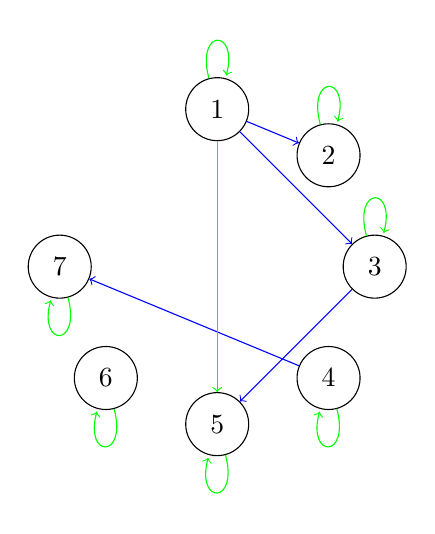
\begin{tikzpicture}[, every node/.style={circle, draw, minimum size=8mm}]
            % Nodes
            \node (1) at (90:2) {1};
            \node (2) at (45:2) {2};
            \node (3) at (0:2) {3};
            \node (4) at (-45:2) {4};
            \node (5) at (-90:2) {5};
            \node (6) at (-135:2) {6};
            \node (7) at (180:2) {7};

            %self loop
            \foreach \i in {1,...,3} {
                \draw[->,green] (\i) edge [loop above] (\i);
            }
            \foreach \i in {4,...,7} {
                \draw[->,green] (\i) edge [loop below] (\i);
            }

            % Edges
            \draw[->,blue] (1) -- (2);
            \draw[->,blue] (1) -- (3);
            \draw[->,blue] (3) -- (5);
            \draw[->,blue] (4) -- (7);
            \draw[->,green] (1) -- (5);
        \end{tikzpicture}
        \caption{First model}
    \end{minipage}
    \quad
    \begin{minipage}[b]{0.45\linewidth}
        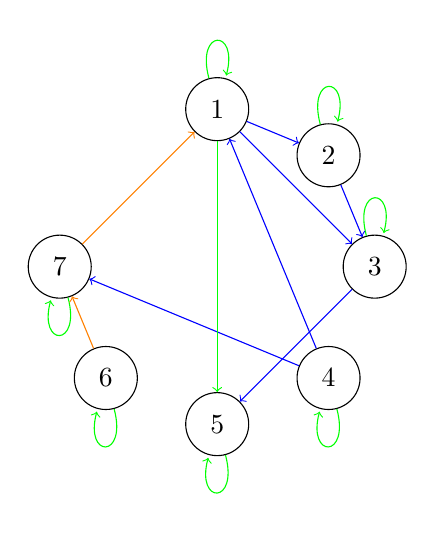
\begin{tikzpicture}[, every node/.style={circle, draw, minimum size=8mm}]
            % Nodes
            \node (1) at (90:2) {1};
            \node (2) at (45:2) {2};
            \node (3) at (0:2) {3};
            \node (4) at (-45:2) {4};
            \node (5) at (-90:2) {5};
            \node (6) at (-135:2) {6};
            \node (7) at (180:2) {7};

            %self loop
            \foreach \i in {1,...,3} {
                \draw[->,green] (\i) edge [loop above] (\i);
            }
            \foreach \i in {4,...,7} {
                \draw[->,green] (\i) edge [loop below] (\i);
            }

            % Edges
            \draw[->,blue] (1) -- (2);
            \draw[->,blue] (1) -- (3);
            \draw[->,blue] (3) -- (5);
            \draw[->,blue] (4) -- (7);
            \draw[->,blue] (2) -- (3);
            \draw[->,green] (1) -- (5);
            \draw[->, orange] (6) -- (7);
            \draw[->, orange] (7) -- (1);
            \draw[->,blue] (4) -- (1);
        \end{tikzpicture}
        \caption{Second model}
    \end{minipage}
    \end{figure}
    
    The first model expresses $T$ as the reflexive transitive closure of the input $E$, whereas the second model expands the first model and adds more additional atoms to a model.
\end{contexample}

Such an ambiguity is not ideal when we want to compute the query results of datalog. Some fragments of logic programming allow multiple models such as answer-set programming, but for datalog, we want a unique model. This is known as the least model. For this, we need to define what least means and show that it exists.

We call a set of ground atoms an \textit{interpretation}. An interpretation represents all true atoms. We want to define the model property from first-order logic for this definition and show then that there exists a least model according to the subset relation.

Recall from first-order logic that $\forall x. \phi(x)$ holds in a structure $\mathcal{A}$ if any element $a \in \mathcal{A}$ we have that $\phi(a)$ holds. As we do not have any function symbols all elements in the universe are constants, so instead of using the universal quantifier we could just create rules by replacing variables with all possible constants.
Formally, this is defined using \textit{groundings} or \textit{instantions} which are functions that map variables to constants. We can apply a grounding $g$ to an atom by replacing every variable $v$ in the terms by $g(v)$ and apply $g$ to a rule by applying it to the head and every atom in the body. At the end of this, we have replaced every variable by a constant and have gained a ground rule. 
The ground program $ground(P)$ of a program $P$ is the set of all ground rules that are the result of applying some grounding to a rule from $P$

We call a ground rule $r$ \textit{true} in an interpretation $I$ if whenever $Body(r)$ is a subset of $I$, then also $Head(r)$ is in $I$.  We call an interpretation $I$ a \textit{model} of a program $P$ if every rule of $ground(P)$ is true in $I$.

So now we have defined models and can define the least model as well. We still need to show that the least model exists for which the following lemma is helpful.

\begin{fact}\label{fact:ModelIntersection}
Let $M_1, M_2$ be two models of a program $P$. Then also $M_1 \cap M_2$ is a model of $P$.
\end{fact}

Therefore the intersection of all models is a model as well and due to the properties of the intersection it is least according to the subset relation. 

In total, we call \[\bigcap_{\text{$M$ is model of $P$}} M\] the \textit{least model} of $P$ and refer to this characterization as the \textit{model-theoretic semantics} of $P$.

\begin{contexample}
    In this example, the first model is actually the least model and the second model is just some other model.

    Therefore the semantic of this program is whenever $Q()$ is given, the reflexive-transitive closure of $E$. 
    If $Q()$ is not given then it is only the reflexive closure.

    Additionally, we see that the rules for $T$ encode general rules whereas the other rules are more a specific input. We might want to reuse these rules for many different instances of $E$, but so far we also need to write a new program.
\end{contexample}

The example raises questions about the reusability of a program. Additionally, we talked in the introduction about database queries but never talked about databases. 

We consider a \textit{database} as a set of ground atoms similar to an interpretation. What is now the semantics of a program $P$ and a database $d$? We simply add every element of $d$ as a fact to $P$ and reuse the previous semantics. Additionally, we can also move all the specific facts from the program into the database and gain a reusable program.
An alternative model definition for a pair of $P$ and $d$ is therefore: An interpretation $I$ is a model for $P$ and $d$ if every ground atom from $d$ is in $I$ and every rule from $ground(P)$ is true in $I$. \cref{fact:ModelIntersection} holds again and we reuse the definition for the database and program case.

Both views are equivalent. We have shown how we can simulate a database by a program. We can simulate the program case with the program and database case by simply using an empty database.

We have now defined the semantics and shown a connection with databases. But this definition is not exactly ideal. In order to find the semantics of a program we would need to check all interpretations and then intersect them all. This is computationally expensive. Is there a simpler way?

We can define a function that computes the least model in a more direct way. For this, we consider the case where only the program $P$ is present.

Consider an interpretation $I$. We call a ground atom $a$ an \textit{immediate consequence} of $I$ if there exists a ground rule $r$ in $ground(P)$ with the head $a$ and $Body(r) \subseteq I$.

The immediate consequence operator $T_P$ adds all immediate consequences to a model. 

\[T_P(I) = \{ a \mid \text {$a$ is an immediate consequence of $I$}\} \]

A fixed point of a function $f$ is an element $k$ such that $f(k) = k$. The repeated application of $T_P$ starting from $\emptyset$ yields a fixed point that is equal to the model-theoretic semantics of a program $P$. 

\begin{contexample}
    We consider again the program $P$. 

    Due to the fact $E(1,3) \leftarrow$, $E(1,3)$ is an immediate consequence of $\emptyset$. Applying $T_P$ again, we have that $T(1,3)$ is an immediate consequence of $\{E(1,3)\}$ due to the rule $T(?x,?y) \leftarrow E(?x, ?y)$ with the grounding 
    
    \[
    g(v) =
    \begin{cases}
        1 & \text{if } v = ?x \\
        3 & \text{else}
    \end{cases}
    \]

    Applying this to every fact, we gain an interpretation $I$ that contains $T(1,3)$ and $T(3,5)$. Then $T(1,5)$ is an immediate consequence of $I$ due to the rule $T(?x, ?z) \leftarrow T(?x,?y) \and T(?y, ?z)$ and the grounding 

    \[
    g'(v) =
    \begin{cases}
        1 & \text{if } v = ?x \\
        3 & \text{if} v = ?y \\
        5 & \text{else}
    \end{cases}
    \]
\end{contexample}

The least fixed-point of $T_P$ is called the \textit{fixed-point semantics} of $P$ and is the basis for most implementations of datalog reasoners. 

Our goal is to explain why an atom is in the datalog result. The third important semantic of datalog helps here. 

A tree $t$ of ground atoms is a proof tree for a ground atom $a$ in a program $P$ and database $d$ if the following three conditions hold:

\begin{enumerate}
    \item the root of $t$ is $a$
    \item for every node $n$ and its children $l$ in $t$ one of the following two conditions holds: 
    \begin{enumerate}
        \item $n \leftarrow l_1 \land ... l_n$ for $l_1,.., l_n \in l$ is a ground rule from $ground(P)$, or
        \item $n$ is a leaf and $n$ is in the database.
    \end{enumerate}
\end{enumerate}

\begin{figure}
    \centering
    \begin{subfigure}[b]{0.45\linewidth}
    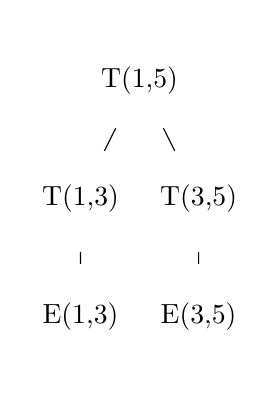
\begin{tikzpicture}[, every node/.style={circle}]
        \node {T(1,5)}
            child {node {T(1,3)}
                child {node {E(1,3)}}
                }
            child {node {T(3,5)}
                child {node {E(3,5)}}};
    \end{tikzpicture}
    \label{prelim:validTree}
    \caption{A valid proof tree}
    \end{subfigure}
    \quad
    \begin{subfigure}[b]{0.45\linewidth}
        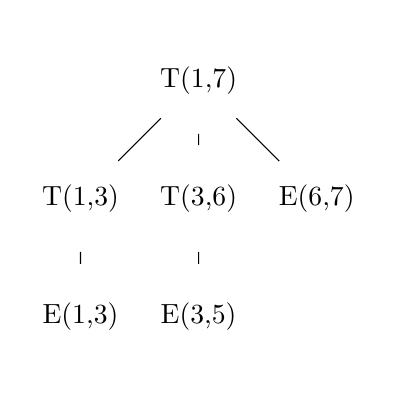
\begin{tikzpicture}[, every node/.style={circle}]
            \node {T(1,7)}
                child {node {T(1,3)}
                    child {node {E(1,3)}}
                    }
                child {node {T(3,6)}
                    child {node {E(3,5)}}}
                child {node {E(6,7)}};
        \end{tikzpicture}
        \caption{An invalid tree}
        \label{prelim:invalidTree}
    \end{subfigure}
    \end{figure}

\begin{contexample}
    The tree in \cref{prelim:validTree} is valid. The leaves of this tree are facts and all other nodes represent ground rules from $ground(P)$ in the previous step.

    The tree in \cref{prelim:invalidTree} is not valid. $E(6,7)$ is neither a fact nor in the database. Additionally there is no rule in $P$ that can result into $T(1,7) \leftarrow T(1,3) \land T(3,6) \land E(6,7)$.
\end{contexample}

The proof-theoretic semantics of a program $P$ and database $d$ is the set of ground atoms that have a valid proof tree. Again this can be shown to be equal to the other semantic definitions. We will formally prove the equality of the proof-theoretic and the model-theoretic semantics of datalog in this work.

\subsection{Certifying algorithms}



\subsection{Lean}

